\documentclass[11pt,a4paper]{article}

\usepackage[margin=20mm,landscape]{geometry}
\usepackage{amsmath,amssymb,amsthm}
\usepackage{graphicx}
\usepackage{booktabs}
\usepackage{array}
\usepackage{xcolor}
\usepackage{microtype}
\usepackage{pdfpages}
\usepackage[colorlinks=true,linkcolor=blue!55!black,urlcolor=blue!55!black]{hyperref}

\definecolor{ink}{HTML}{0B0B0B}
\definecolor{soft}{HTML}{52514E}
\definecolor{accent}{HTML}{2A78D6}
\definecolor{warn}{HTML}{D03B3B}

\newcommand{\T}{^{\mathsf{T}}}
\newcommand{\Lp}{L^{+}}
\newcommand{\note}[1]{{\color{soft}\small #1}}

% !TeX root = ../pipeline.tex
\newcommand{\gnb}{754}
\newcommand{\gne}{980}
\newcommand{\gnlines}{755}
\newcommand{\gntx}{225}
\newcommand{\gnwind}{157}
\newcommand{\gnwindgen}{425}
\newcommand{\gnPtdfEntries}{738,920}
\newcommand{\gnLpEntries}{568,516}
\newcommand{\grank}{750}
\newcommand{\gnullity}{4}
\newcommand{\growsum}{3.6e-10}
\newcommand{\gLone}{2.3e-10}
\newcommand{\gpsum}{1.6e-12}
\newcommand{\gpeffsum}{1.3e-12}
\newcommand{\gresid}{2.1e-09}
\newcommand{\gKdense}{0.27}
\newcommand{\gLdense}{0.46}
\newcommand{\gLpdense}{99.2}
\newcommand{\gnshift}{2}
\newcommand{\gshiftdeg}{17}
\newcommand{\gsnap}{2030-01-16 16:00:00}
\newcommand{\gworst}{1122-1742-1}
\newcommand{\gncong}{6}
\newcommand{\gncongtx}{0}
\newcommand{\gbmin}{-21638.3}
\newcommand{\gbmax}{1754386.0}
\newcommand{\gptdfmin}{-1.2093}
\newcommand{\gptdfmax}{1.0105}
\newcommand{\gwinb}{10}
\newcommand{\gwine}{6}
\newcommand{\gnnonwind}{597}
\newcommand{\gnwindentries}{153,860}
\newcommand{\gcommute}{0.0e+00}

% !TeX root = ../pipeline.tex
\newcommand{\pN}{20,203}
\newcommand{\pOut}{432}
\newcommand{\pTau}{0.05}
\newcommand{\pTol}{0.1}
\newcommand{\pEirCleared}{92.0}
\newcommand{\pEirBrokeEvents}{642}
\newcommand{\pEirBrokeLines}{873}
\newcommand{\pEirMedNodes}{18}
\newcommand{\pEirCommonMW}{822,672}
\newcommand{\pOvlBrokeEvents}{1,085}
\newcommand{\pOvlBrokeLines}{1,354}
\newcommand{\pVetoCleared}{89.9}
\newcommand{\pVetoBrokeEvents}{0}
\newcommand{\pVetoBrokeLines}{0}
\newcommand{\pVetoMedNodes}{1}
\newcommand{\pVetoCommonMW}{626,626}
\newcommand{\pSavedMW}{196,045}
\newcommand{\pSavedPct}{23.8}
\newcommand{\pLpCleared}{99.8}
\newcommand{\pLpFeasible}{99.8}
\newcommand{\pTrips}{1,308}
\newcommand{\pTripsOutages}{432}
\newcommand{\pTripsCircuits}{58}
\newcommand{\pMedGroupOverlap}{61}
\newcommand{\pMedGroupEir}{42}
\newcommand{\pVetoedFromEir}{5,100}
\newcommand{\pVetoedFromEirPct}{10.0}
\newcommand{\pWindN}{157}
\newcommand{\pWindFleetMW}{12,701}
\newcommand{\pMinCutEvents}{6}
\newcommand{\pRareN}{119}
\newcommand{\pRarePct}{75.8}
\newcommand{\pRareMW}{8,367}
\newcommand{\pRareFleetPct}{65.9}
\newcommand{\pMedEventsPct}{0.52}
\newcommand{\pMedKeptPct}{99.61}
\newcommand{\pTopFivePct}{46}
\newcommand{\pTopTenPct}{59}
\newcommand{\pTopTwentyPct}{72}
\newcommand{\pTotalCutMW}{921,085}
\newcommand{\pTotalOfferedMW}{108,051,058}
\newcommand{\pOverallCutPct}{0.85}
\newcommand{\pCascN}{250}
\newcommand{\pNothingLost}{814}
\newcommand{\pNothingSpread}{250}
\newcommand{\pNothingIsl}{169}
\newcommand{\pCEirLost}{309}
\newcommand{\pCEirSpread}{137}
\newcommand{\pCEirIsl}{72}
\newcommand{\pCVetoLost}{261}
\newcommand{\pCVetoSpread}{119}
\newcommand{\pCVetoIsl}{55}
\newcommand{\pCLpLost}{38}
\newcommand{\pCLpSpread}{25}
\newcommand{\pCLpIsl}{7}


\pagestyle{empty}

\begin{document}

% ---- title ---------------------------------------------------
\thispagestyle{empty}
\vspace*{\fill}
\begin{center}
{\LARGE\bfseries Tackling the problem of constraint group construction\\[3mm]
to reduce wind energy waste and defend against cascading outages}

\vspace{10mm}
{\large Team 6}
\end{center}
\vspace*{\fill}
\newpage

% ---- teammate slides, shown first ----------------------------
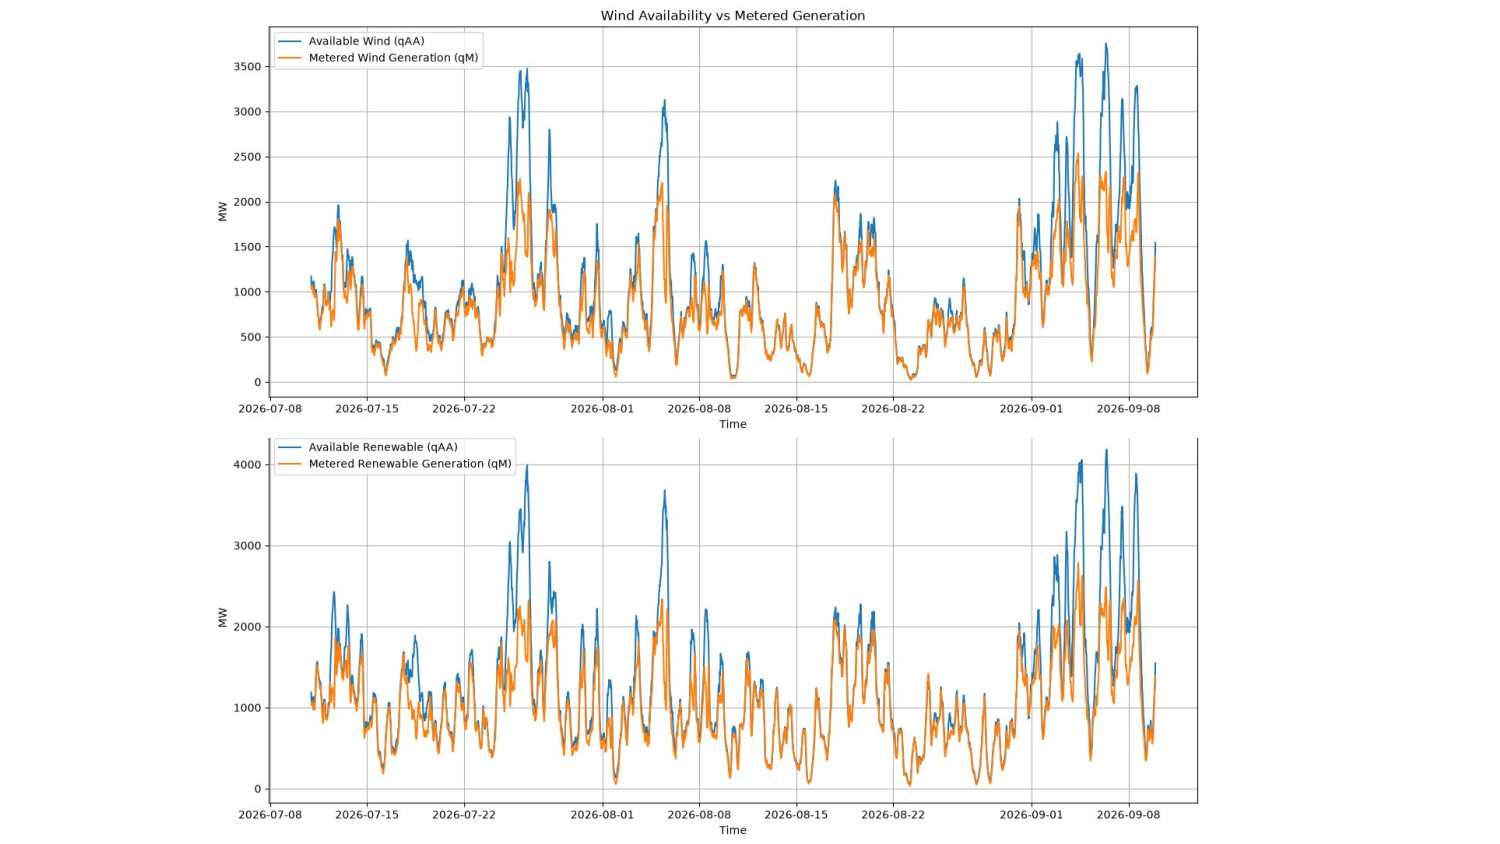
\includepdf[pages=-,fitpaper=true]{figures/vilmos.pdf}

% ===============================================================
\section{The shift factor, as it is used today}

For a branch $e$ and a generator at node $n$:
\begin{equation}
  \text{SF}_{e,n} \;=\; \frac{\Delta f_e}{\Delta P_n}.
  \label{eq:sf}
\end{equation}

Two properties define how it is used:

\medskip
\textbf{It is transmission-line specific.} One number describes one branch
against one generator. A constraint group is built by computing a column of
these for a single congested circuit.

\medskip
\textbf{It is empirical.} [WDT] (Appendix 2, p.\,71) obtains it by
perturbation: move one generator by a fixed amount, re-run the load flow, read
the change in branch current. One solve per number.

% ===============================================================
\newpage
\section{Sensitivity: a new way of looking at it}

\begin{equation}
  S_{e,n} \;=\; \text{PTDF}_{e,n}\cdot\operatorname{sign}(f_e).
  \label{eq:sens}
\end{equation}

The same physical quantity as \eqref{eq:sf}, with the sign re-pointed along
each branch's real direction of flow, so that \textbf{positive always means
relief}.

\medskip
Without the correction a positive entry means ``flow increases in the
branch's stored \texttt{bus0}$\rightarrow$\texttt{bus1} direction'', which is
overload on one branch and relief on another. With it, one row may be ranked,
and two rows may be added.

\medskip
It is \textbf{dimensionless}, MW off the branch per MW curtailed at the
node, so entries from different branches are directly comparable.

% ===============================================================
\newpage
\section{How to get to \texorpdfstring{$S$}{S}: \texorpdfstring{$K$, $B$, $L$}{K, B, L}}

\textbf{$K$, incidence, $\gnb \times \gne$.} Topology only. Column $e$ has
exactly two non-zeros: $+1$ at the branch's \texttt{bus0}, $-1$ at its
\texttt{bus1}.
\[
  K_{ie} = \begin{cases}
    +1 & i = \text{bus0}(e)\\
    -1 & i = \text{bus1}(e)\\
    0  & \text{otherwise.}
  \end{cases}
\]

\textbf{$B$, susceptance, $\gne \times \gne$ diagonal.} Electrical strength
only: $B_{ee} = b_e = 1/x_e$, from the per-unit reactance.

\medskip
\textbf{$L = KBK\T$, the weighted Laplacian, $\gnb \times \gnb$.} Topology
and strength combined, and the matrix that must be inverted:
\begin{equation}
  L\theta \;=\; p .
\end{equation}

\medskip
\note{\textbf{Why any of this is linear.} The AC equations are not. The DC
approximation holds bus voltages at $1$ p.u., takes $r \ll x$ so losses
vanish, and takes angle differences small so
$\sin(\theta_i-\theta_j)\approx\theta_i-\theta_j$. Flow is then exactly linear
in the angle difference, $f_e = b_e(\theta_i-\theta_j)$. That is the whole
reason a closed-form sensitivity exists at all.}

% ===============================================================
\newpage
\section{The matrices themselves}

\begin{center}
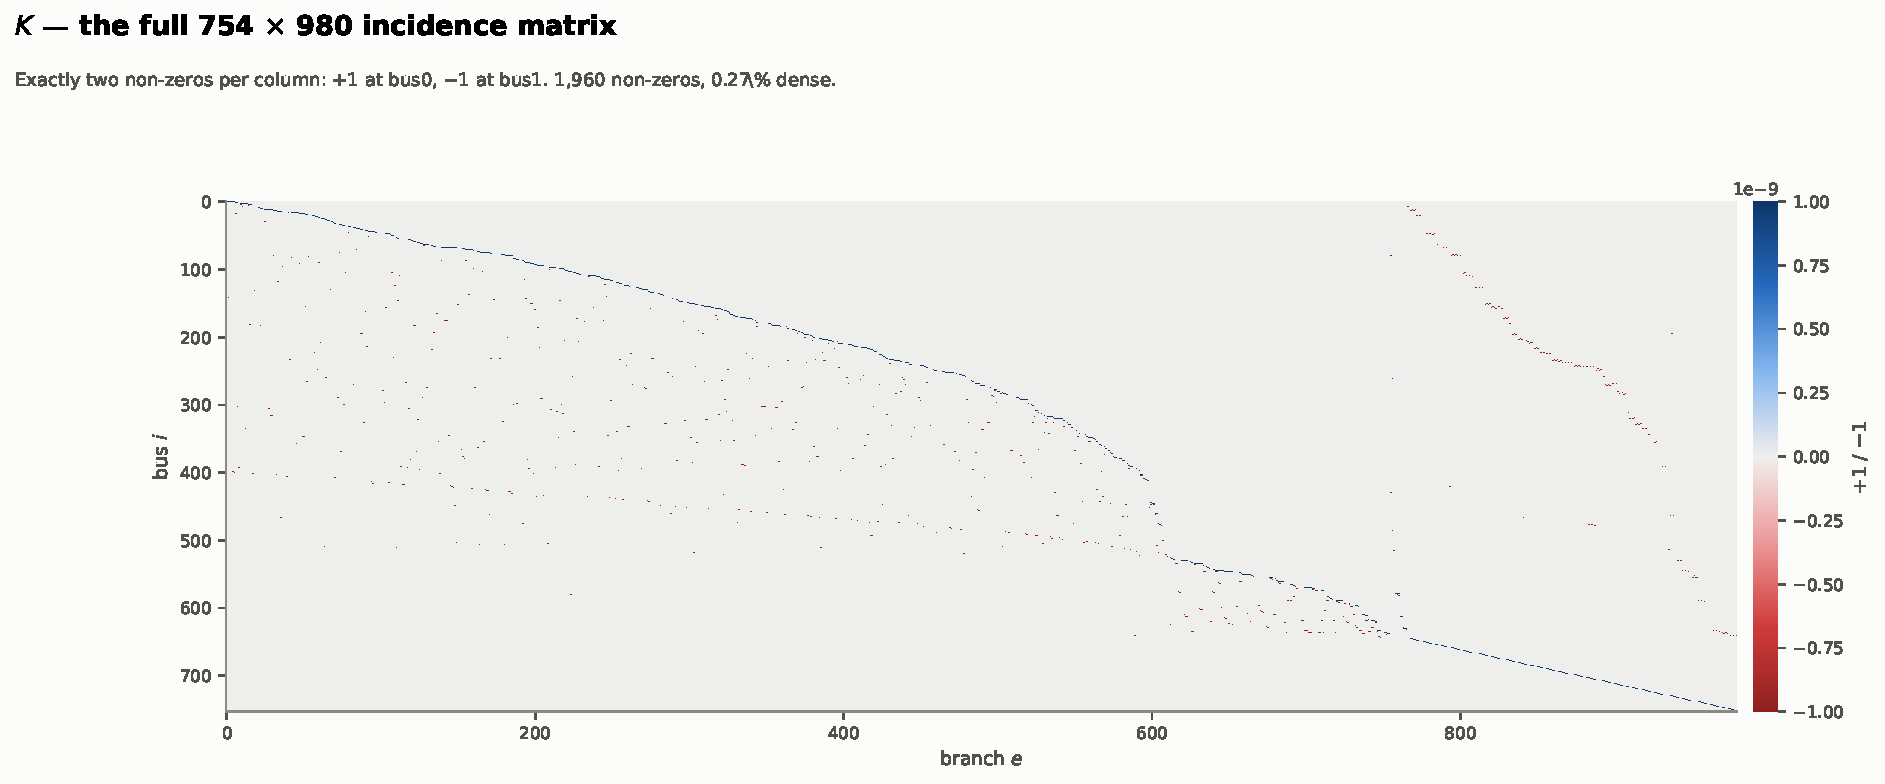
\includegraphics[height=0.295\textheight]{figures/m_K}\\[1mm]
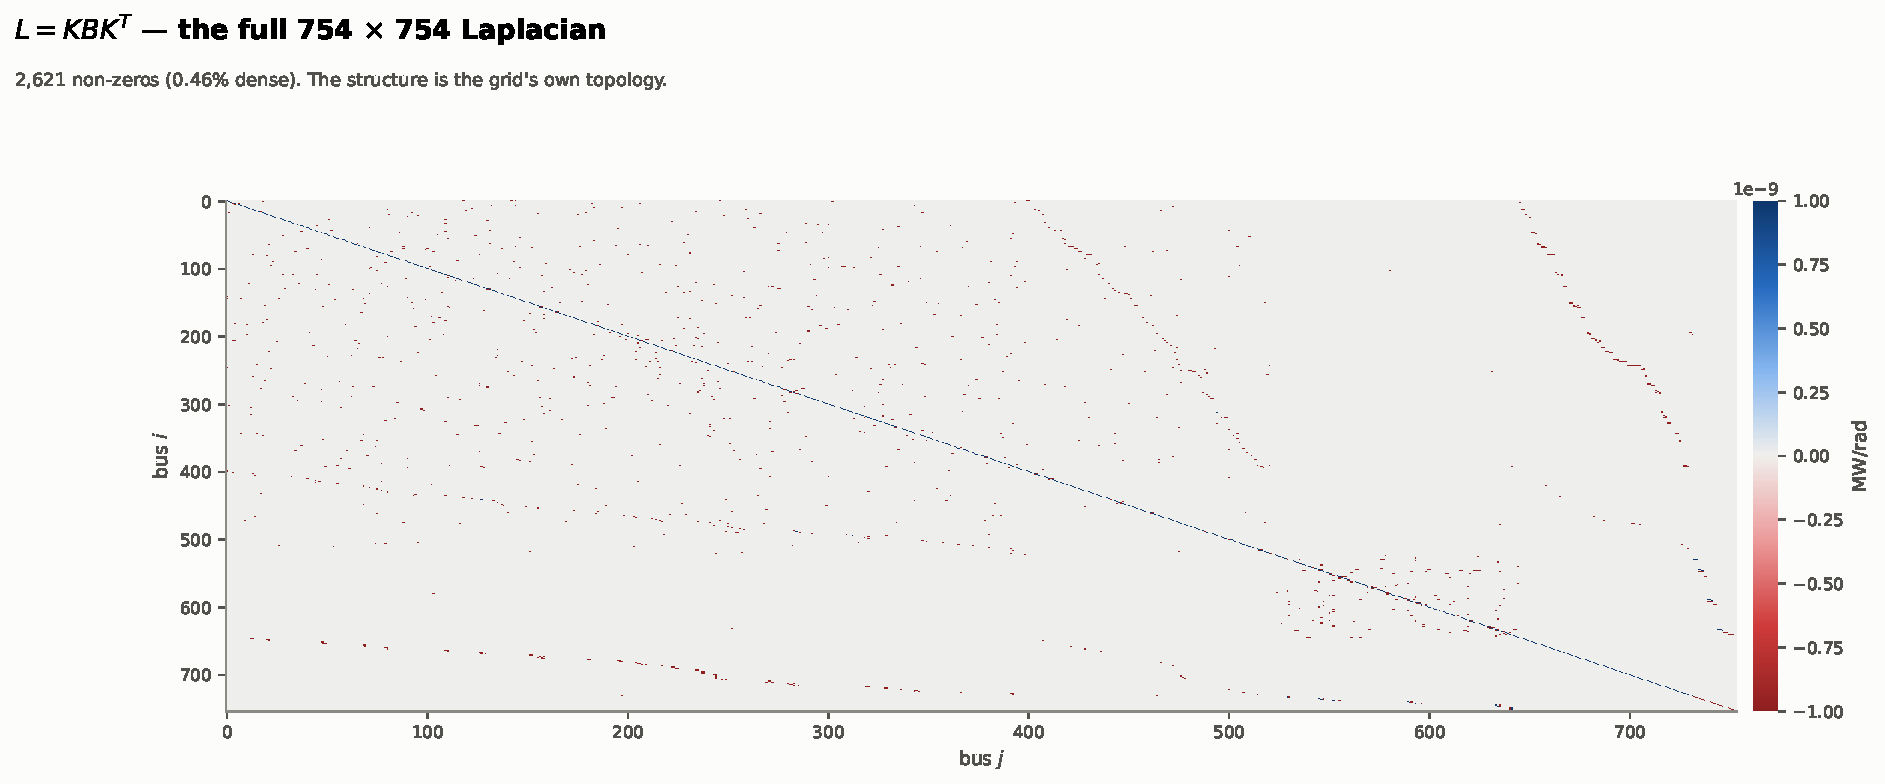
\includegraphics[height=0.295\textheight]{figures/m_L}\\[1mm]
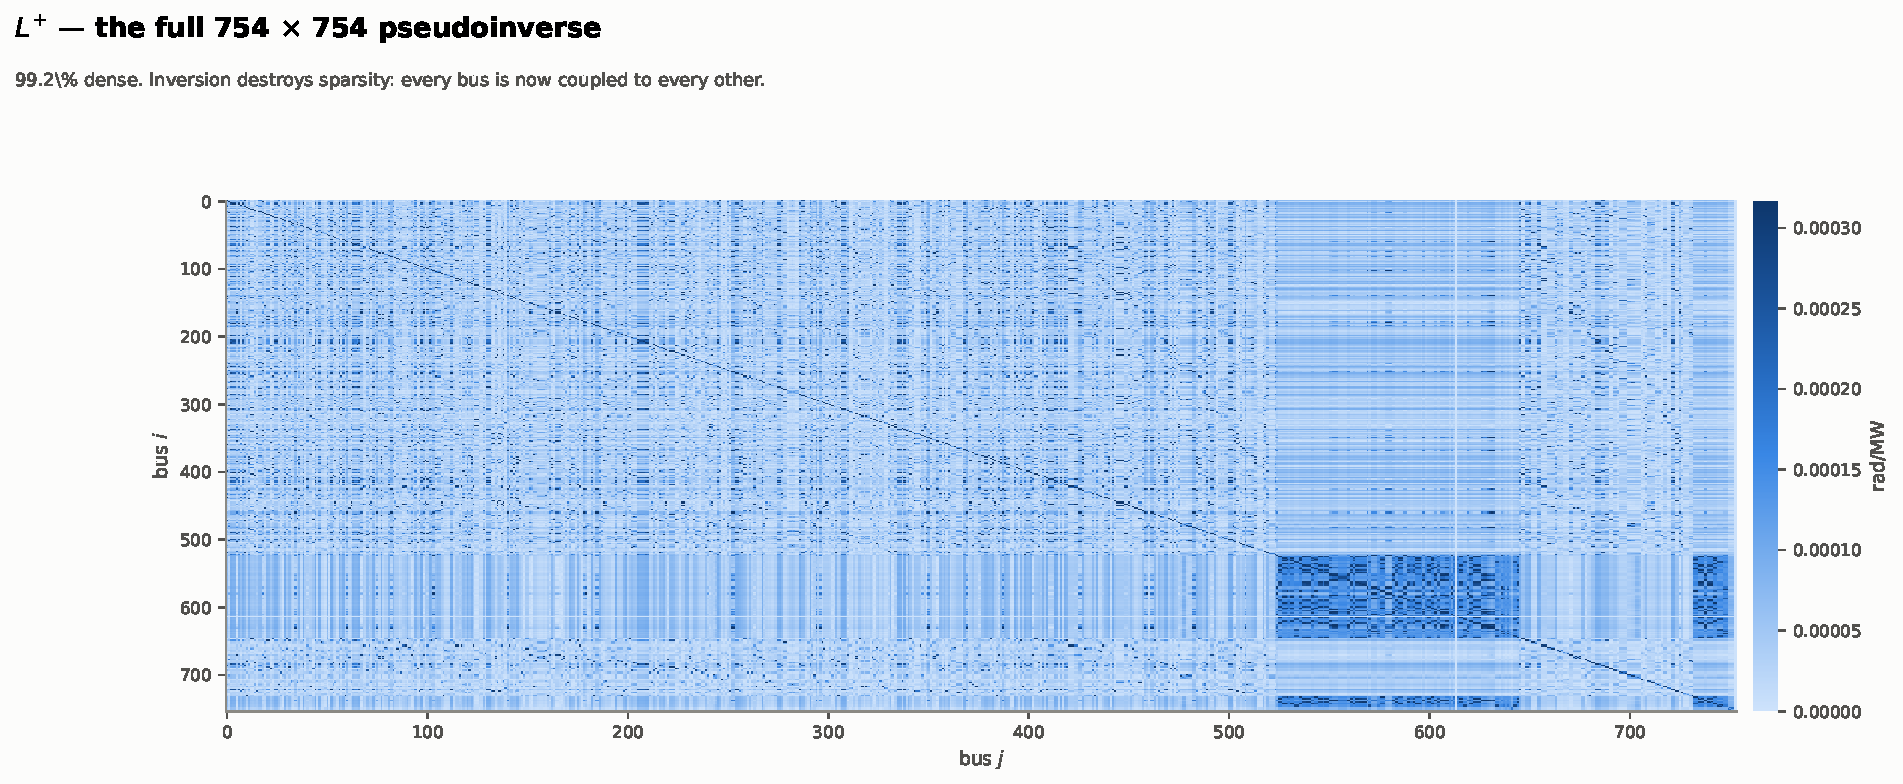
\includegraphics[height=0.295\textheight]{figures/m_Lp}
\end{center}

% ===============================================================
\newpage
\section{The PTDF}

\begin{equation}
  \text{PTDF} \;=\; B K\T \Lp,
  \qquad \gne \times \gnb, \quad \gnPtdfEntries \text{ entries}.
  \label{eq:ptdf}
\end{equation}

$\text{PTDF}_{e,n}$ is the flow appearing on branch $e$ when $1$\,MW is
injected at bus $n$ and withdrawn across the slack.

\begin{center}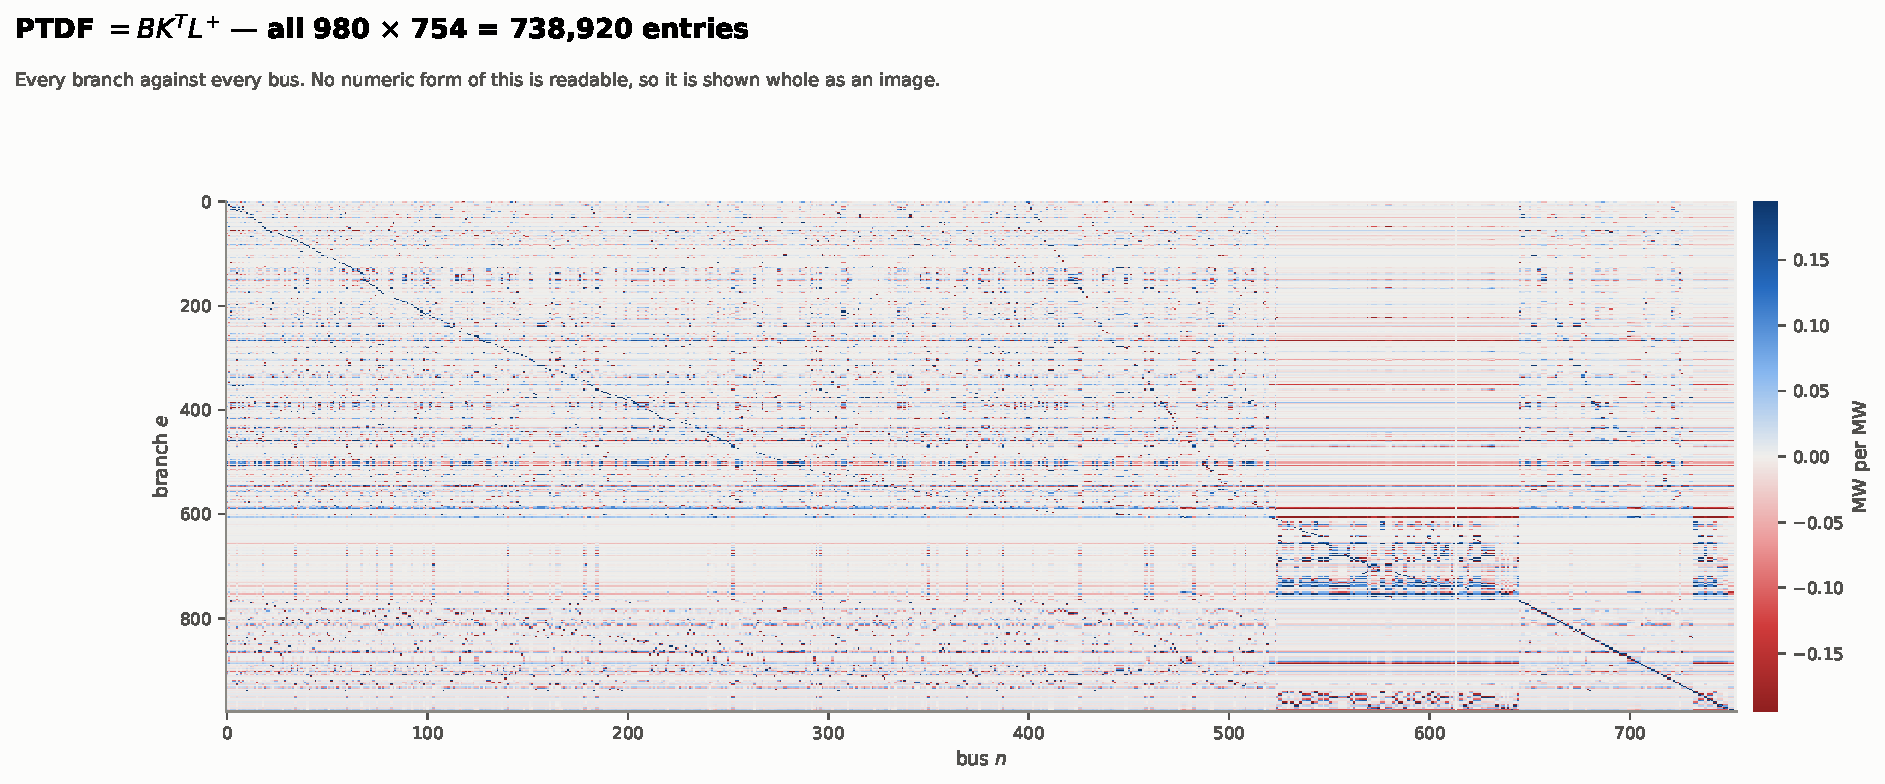
\includegraphics[width=0.86\linewidth]{figures/m_PTDF}\end{center}


% ===============================================================
\newpage
\section{The sensitivity matrix}

Only one quantity in the pipeline moves hour to hour: the direction of flow.
\begin{equation}
  p_{\text{eff}} = p + KB\varphi, \qquad
  f = \text{PTDF}\cdot p_{\text{eff}} - B\varphi, \qquad
  S_{e,:} = \text{PTDF}_{e,:}\operatorname{sign}(f_e).
\end{equation}

\begin{center}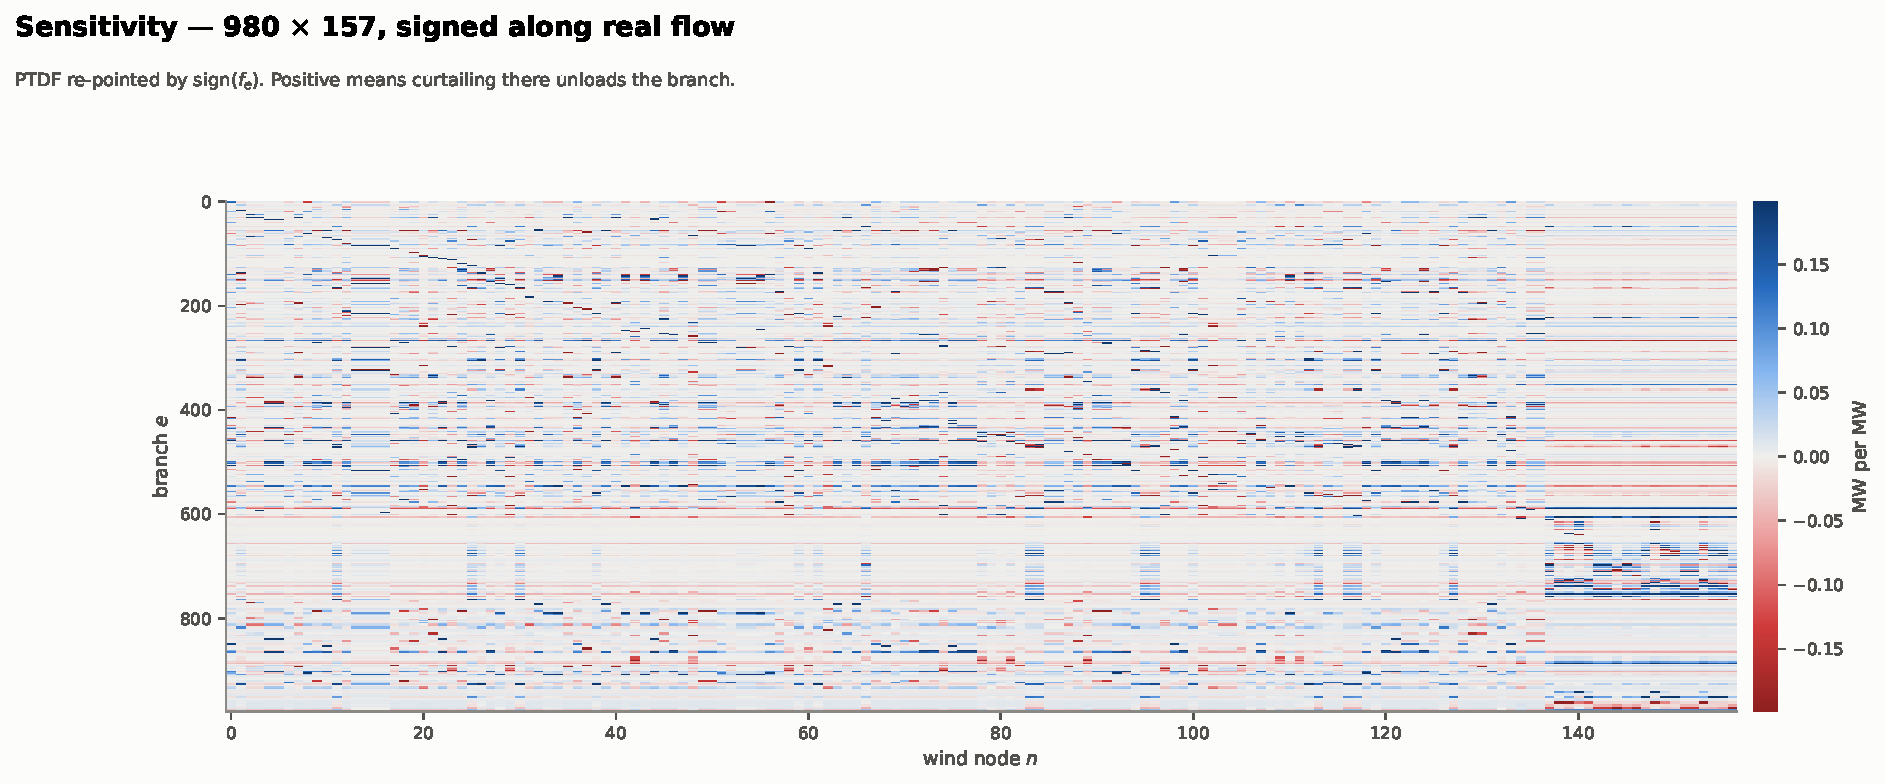
\includegraphics[width=0.86\linewidth]{figures/m_sens}\end{center}

\begin{center}\small
\begin{tabular}{ll}
\toprule
positive & curtailing at that wind node \textbf{unloads} the branch\\
negative & curtailing at that wind node \textbf{loads it further}\\
\bottomrule
\end{tabular}
\end{center}

\medskip
\note{$\varphi$ holds the phase shifts of the $\gnshift$ phase-shifting
transformers. Dropping the $-B\varphi$ term puts the flow, and therefore the
sign, and therefore every entry of $S$, wrong on those branches.}

% ===============================================================
\newpage
\section{In practice, only a small set of lines is congested}

Of $\gne$ branches, only a handful reach their rating at any hour of the week,
and several of those are transformers, which a lines-only model would miss
entirely.

\begin{center}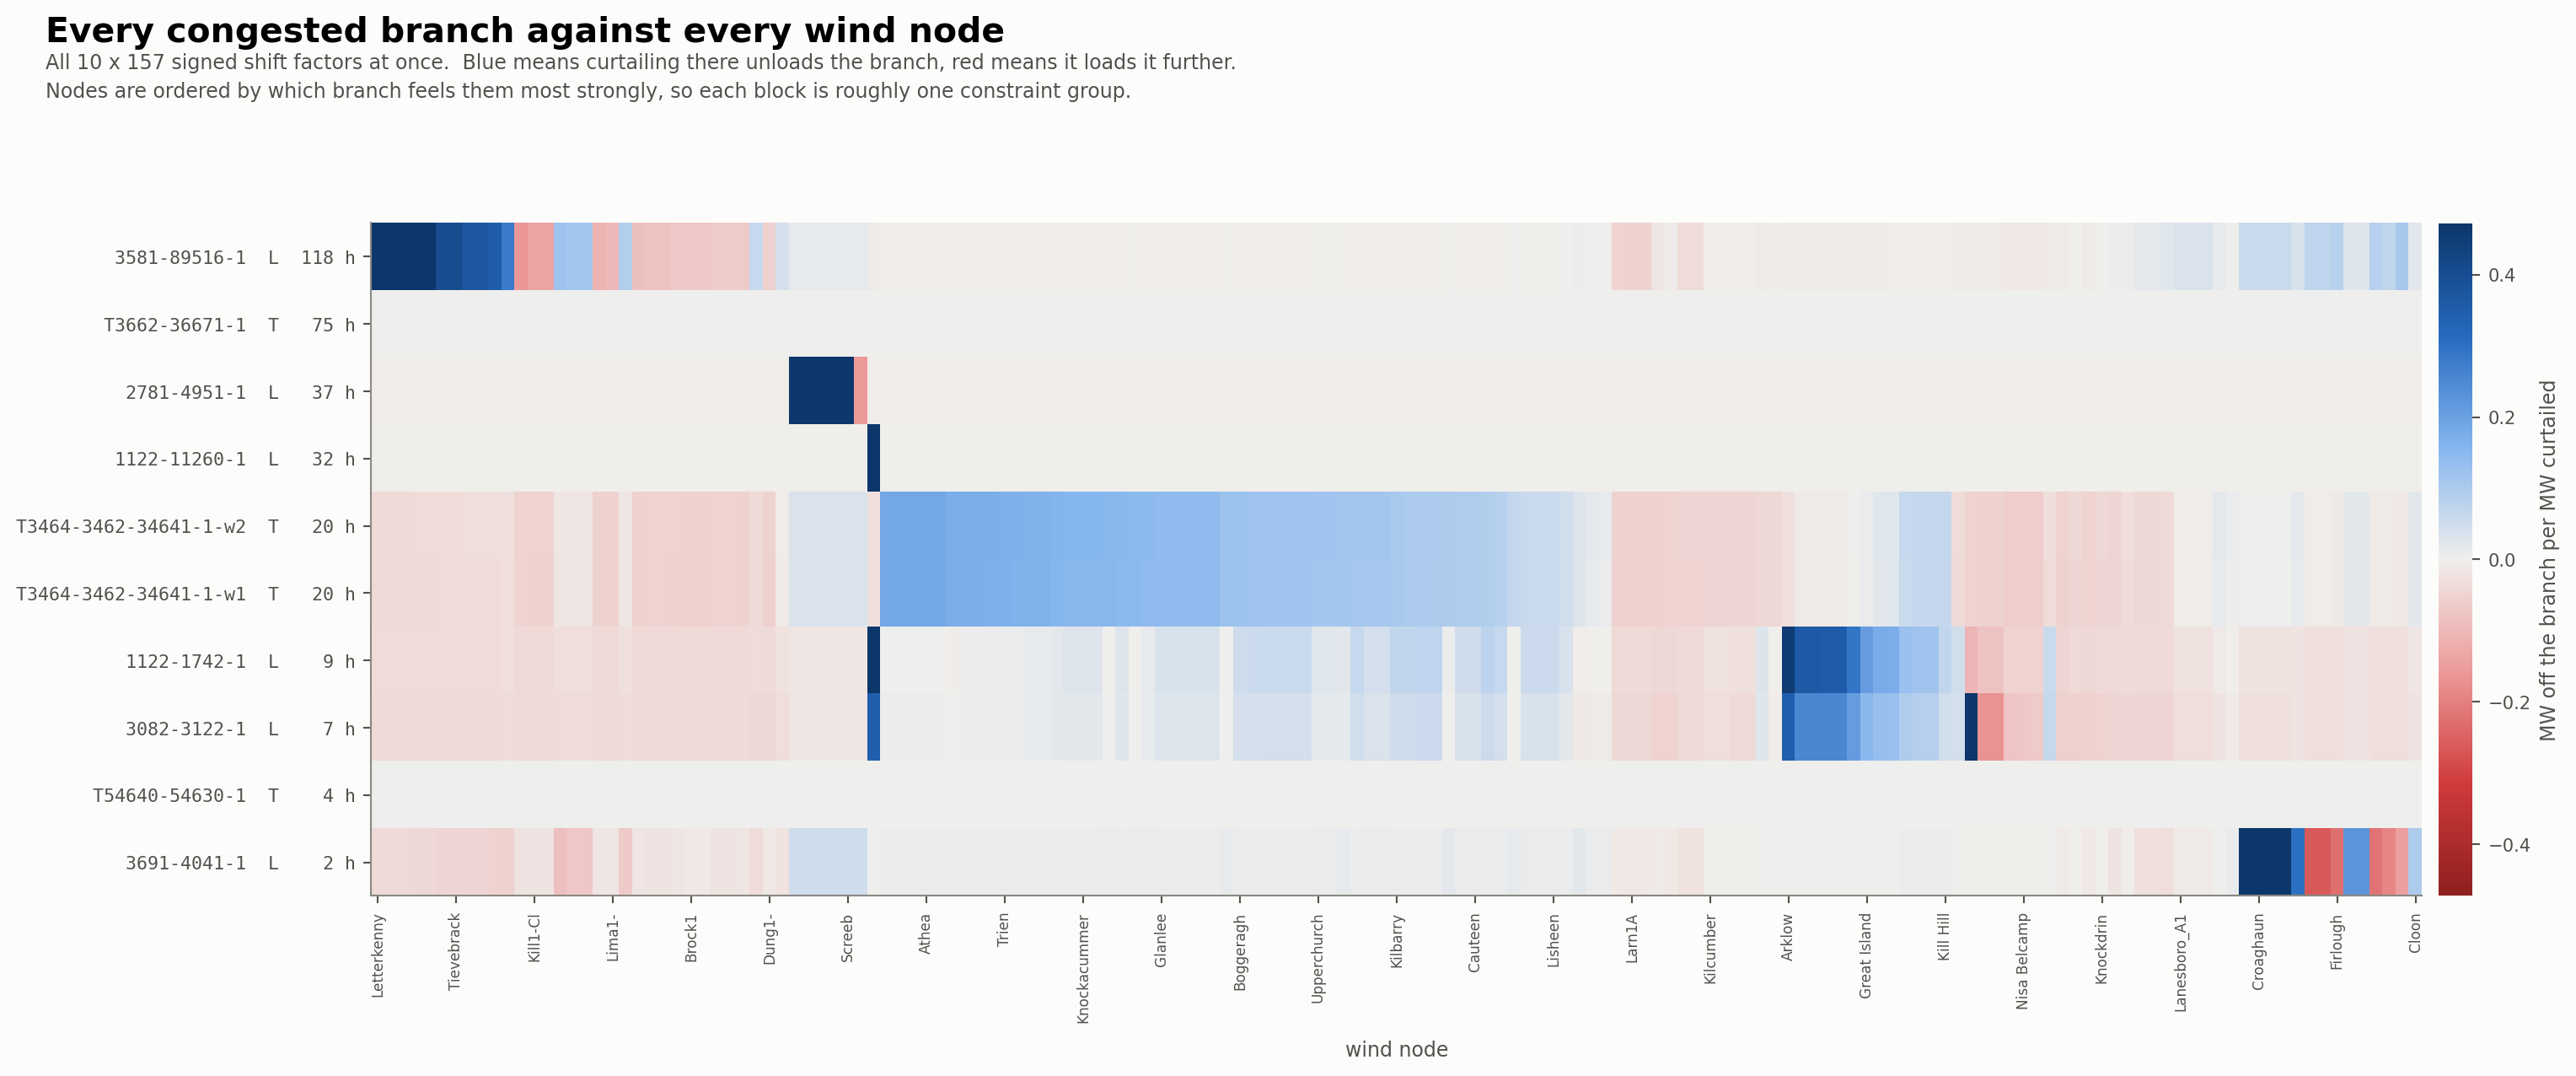
\includegraphics[width=\linewidth]{figures/f_heatmap}\end{center}

\medskip
Every constraint question in the rest of this document is a question about
these rows. The remaining rows exist, are exact, and are never needed until the
network changes, which is what an outage is.

% ===============================================================
\newpage
\section{Net sensitivity: a constraint group that cannot break what it did not look at}

\subsection*{The group, as it is drawn today}

\begin{equation}
  \text{group}(e) \;=\; \{\, n : S_{e,n} \,\ge\, \tau \,\},
  \qquad \tau = \pTau .
\end{equation}

\subsection*{Sensitivities add. Net sensitivity is nothing more than that.}

If several branches are over their rating at once, a node's total usefulness is
its sensitivities to each of them, summed:
\begin{equation}
  S_{\text{net}}(n) \;=\; \sum_{e\,\in\,\text{Over}} S_{e,n},
  \qquad \text{Over} = \{\, e : |f_e| > s_e \,\}.
  \label{eq:netsens}
\end{equation}

\subsection*{The critical principle}

\textbf{No dispatch down of a node may cause an overload on any other branch.}

\begin{center}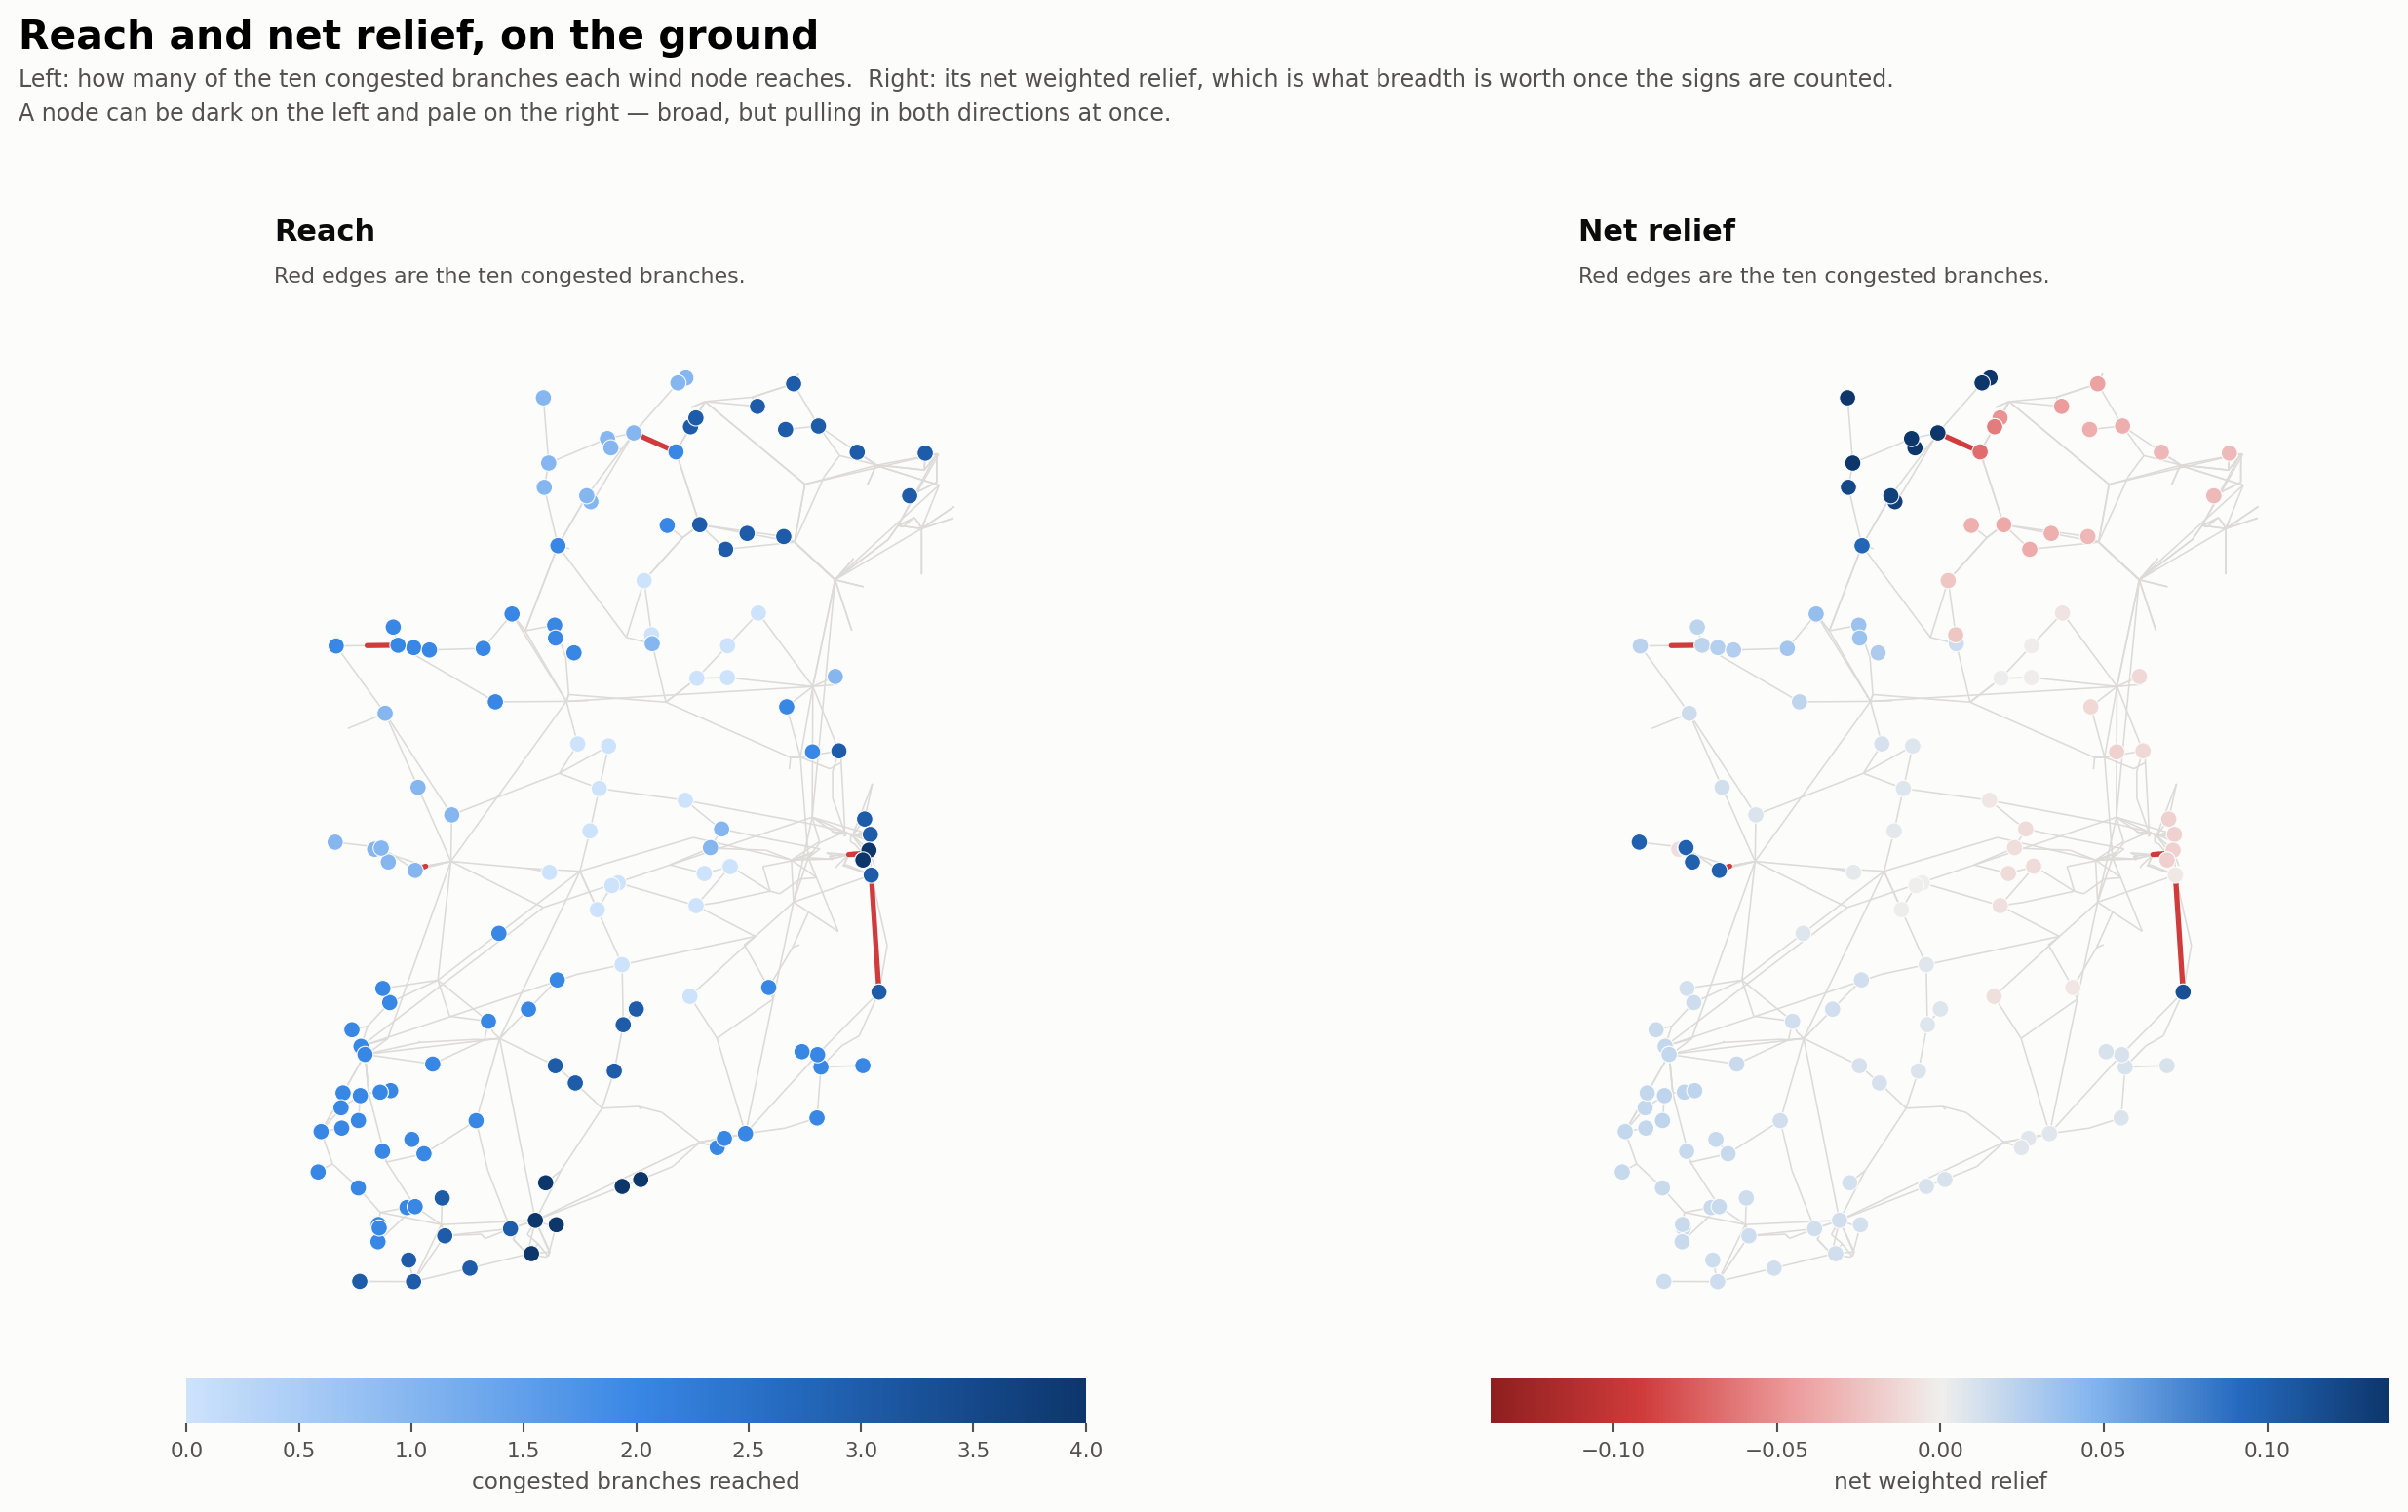
\includegraphics[width=0.92\linewidth]{figures/f_reach}\end{center}
\note{Left: how many congested branches each wind node reaches. Right: its net
weighted relief, \eqref{eq:netsens}. A node dark on the left and pale on the
right is broad but pulling both ways at once, which counting rows cannot
distinguish and summing them can.}

% ===============================================================
\newpage
\section{Doing this for every N--1 contingency}

\textbf{The groups are fixed.} Membership is read off $S$, which is topology
and reactance only, so it does not move with the hour or the weather. The group
for every single-branch outage is built once, offline, and looked up:
\pTripsOutages\ outages, \pTripsCircuits\ distinct circuits ever at risk,
\pTrips\ lookup rows.

\medskip
\textbf{Most of the fleet is almost never in one.} Across all \pN\ events,
\pRareN\ of \pWindN\ nodes, \pRareFleetPct\% of installed capacity, are
dispatched down in under $1\%$ of them. The median node keeps
\pMedKeptPct\% of everything it offers, and over the whole study only
\pOverallCutPct\% of all wind offered is curtailed.

\medskip
For those generators a constraint group binds on a handful of hours a year. It
is not a standing limit on output, and they run at full power essentially all
the time.

\medskip
\textbf{And a few of these outages do not stop at one circuit.}

% ===============================================================
\newpage
\section{Another application: stopping cascading outages}

Most single-branch outages are absorbed. Flows redistribute and nothing else
reaches its rating. A small number are not: the first trip pushes other
elements over their limits, those trip in turn, and the failure propagates.

\medskip
This is where the two constraint groups separate. A group drawn from one row can
relieve the congested circuit while pushing a healthy one over, which starts the
next link in the chain. A group built under the critical principle cannot.

\medskip
\begin{center}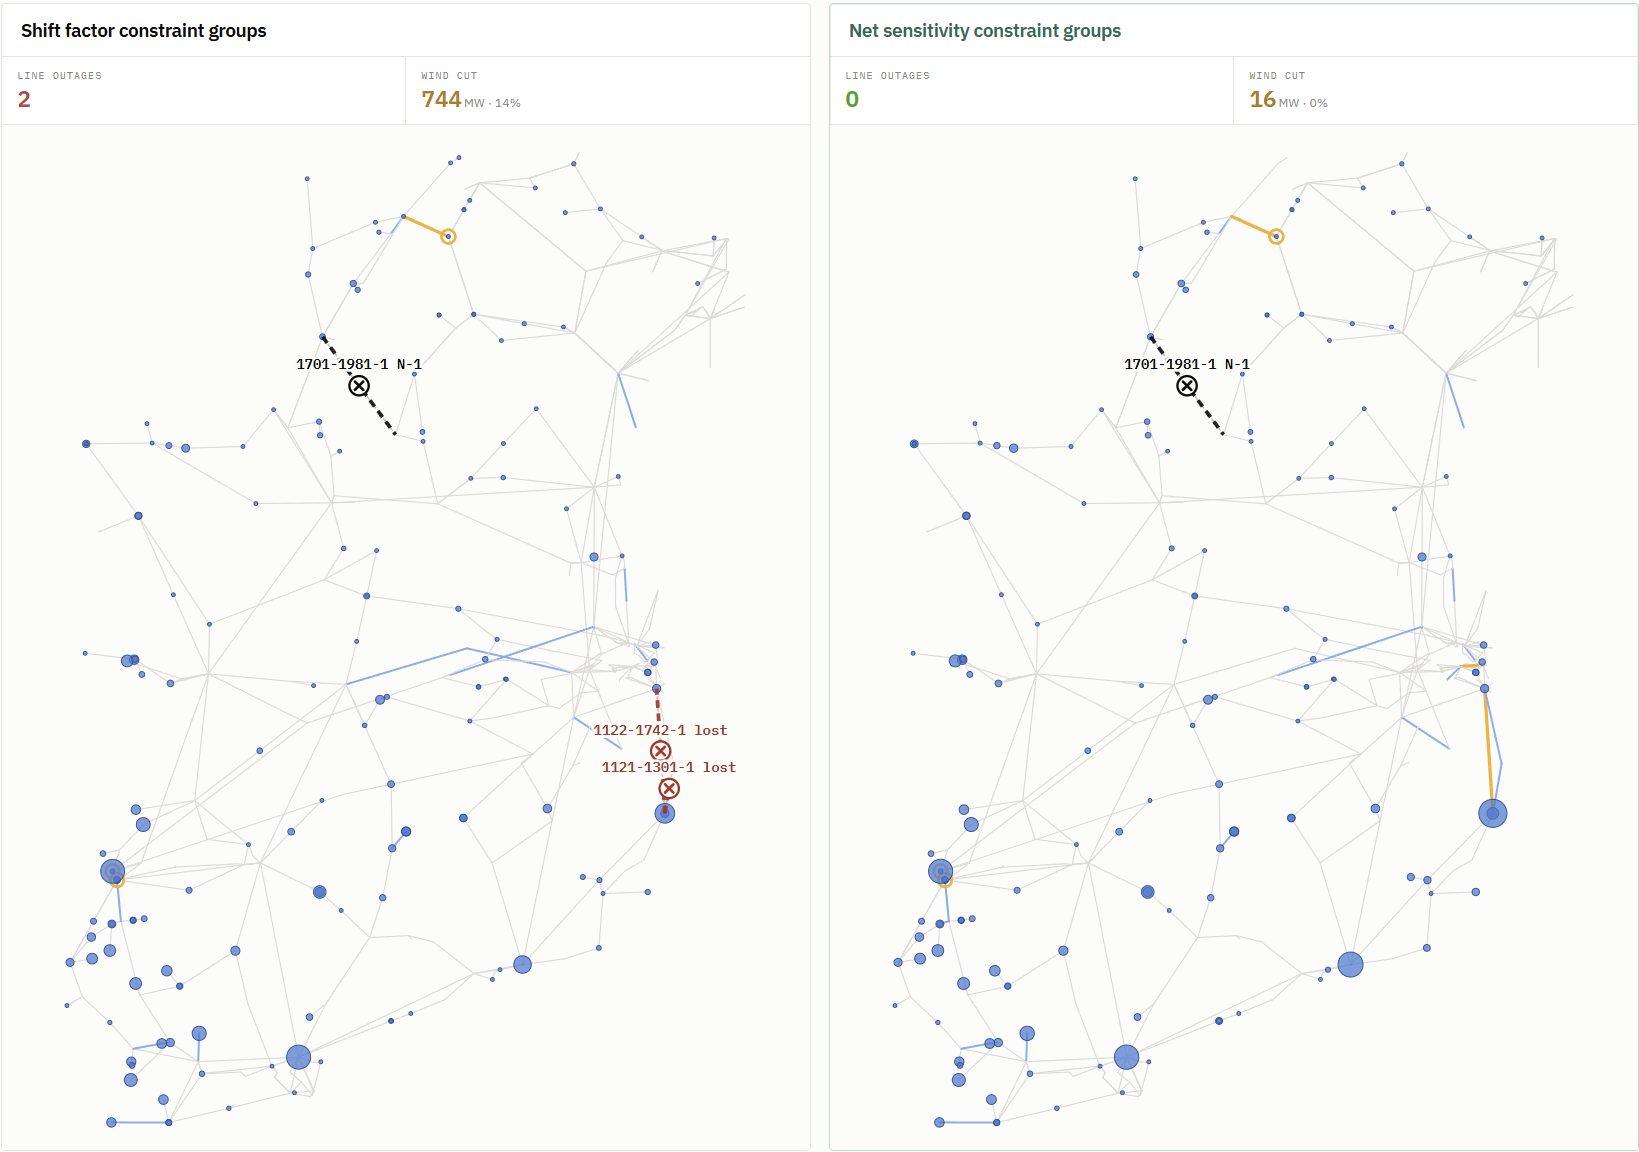
\includegraphics[width=\linewidth]{figures/f_cascade}\end{center}

% ---- teammate slides, shown last -----------------------------
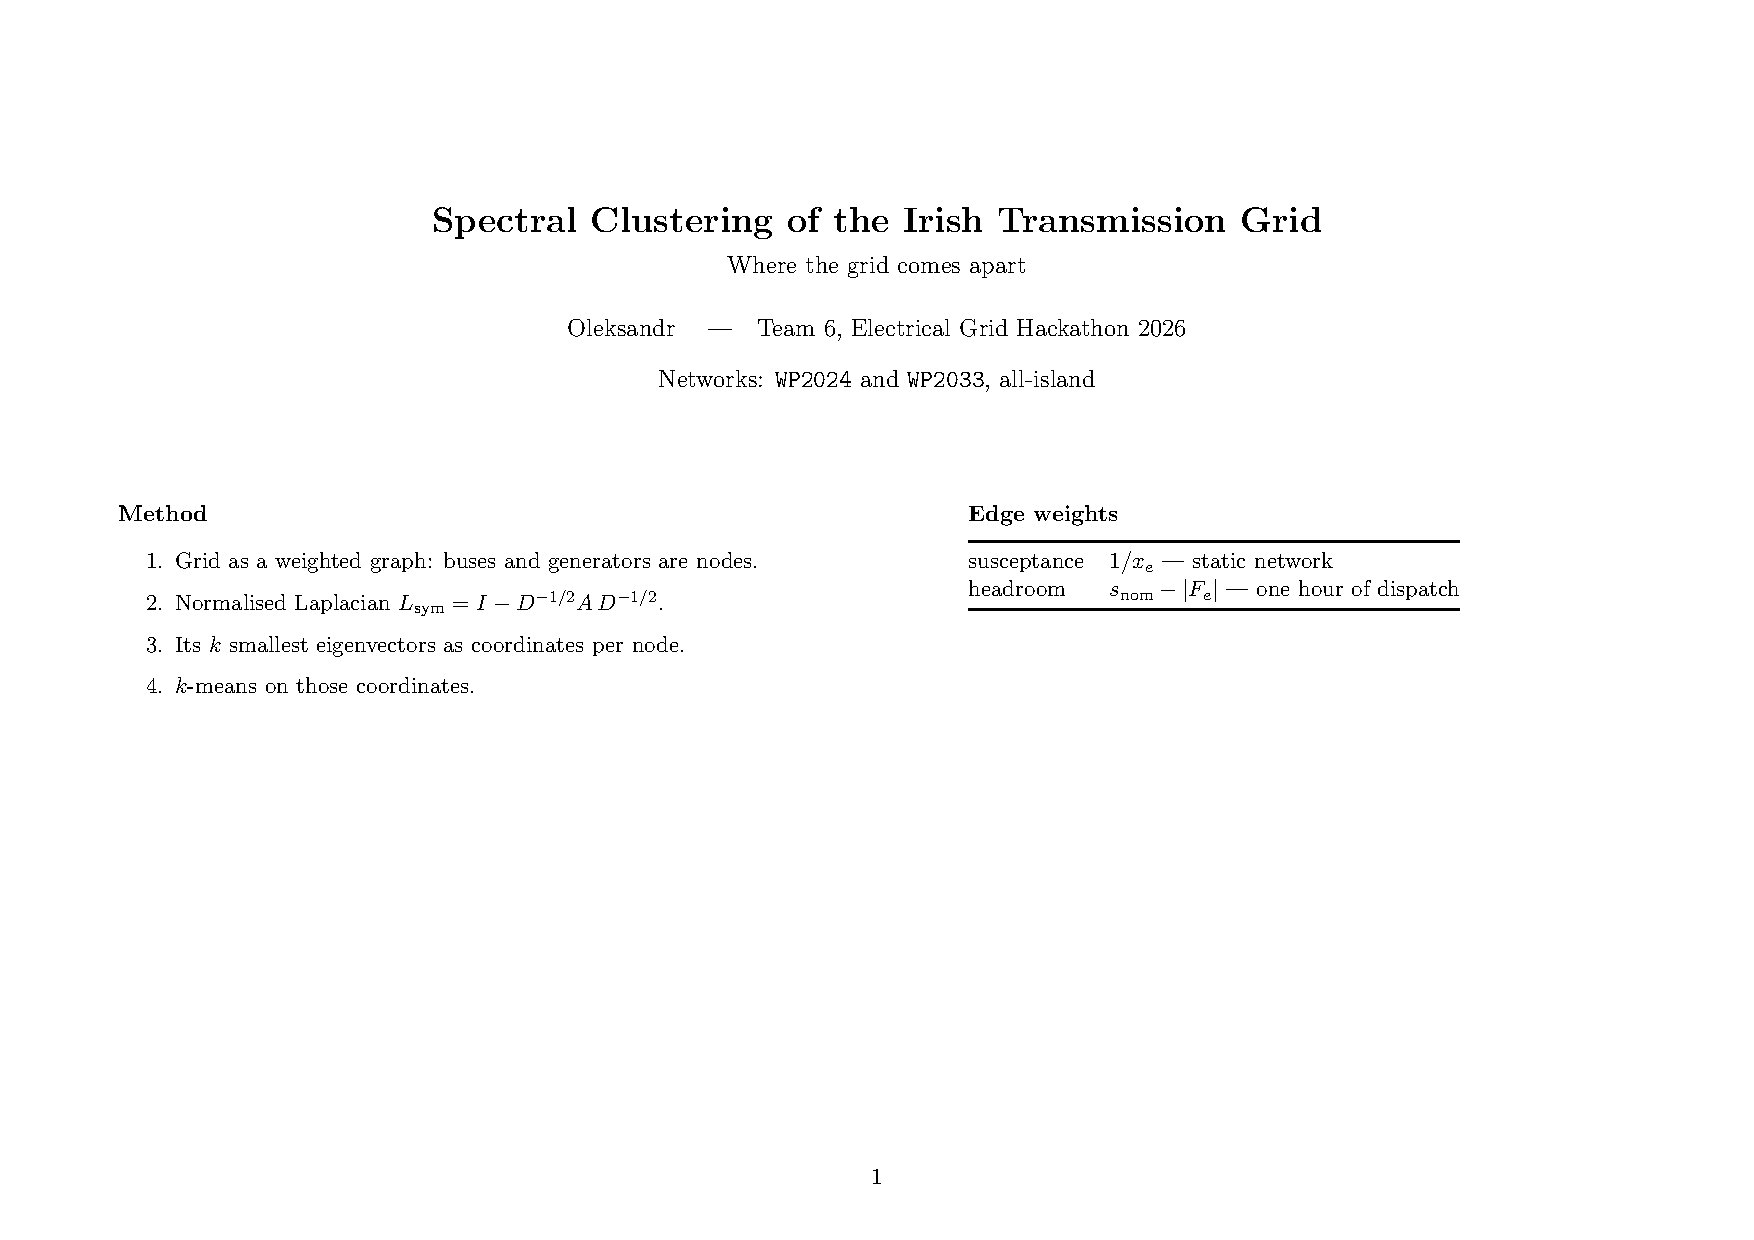
\includepdf[pages=-,fitpaper=true]{figures/oleksandr.pdf}

\end{document}
